\section{Contributions}
The listing of authors is in alphabetical order based on their last names. 
\begin{multicols}{4}
Yifan Bai\\
Yiping Bao\\
Y. Charles\\
Cheng Chen\\
Guanduo Chen\\
Haiting Chen\\
Huarong Chen\\
Jiahao Chen\\
Ningxin Chen\\
Ruijue Chen\\
Yanru Chen\\
Yuankun Chen\\
Yutian Chen\\
Zhuofu Chen\\
Jialei Cui\\
Hao Ding\\
Mengnan Dong\\
Ang'ang Du\\
Chenzhuang Du\\
Dikang Du\\
Yulun Du\\
Yu Fan\\
Yichen Feng\\
Kelin Fu\\
Bofei Gao\\
Chenxiao Gao\\
Hongcheng Gao\\
Peizhong Gao\\
Tong Gao\\
Yuyao Ge\\
Shangyi Geng\\
Qizheng Gu\\
Xinran Gu\\
Longyu Guan\\
Haiqing Guo\\
Jianhang Guo\\
Xiaoru Hao\\
Tianhong He\\
Weiran He\\
Wenyang He\\
Yunjia He\\
Chao Hong\\
Hao Hu\\
Yangyang Hu\\
Zhenxing Hu\\
Weixiao Huang\\
Zhiqi Huang\\
Zihao Huang\\
Tao Jiang\\
Zhejun Jiang\\
Xinyi Jin\\
Yongsheng Kang\\
Guokun Lai\\
Cheng Li\\
Fang Li\\
Haoyang Li\\
Ming Li\\
Wentao Li\\
Yang Li\\
Yanhao Li\\
Yiwei Li\\
Zhaowei Li\\
Zheming Li\\
Hongzhan Lin\\
Xiaohan Lin\\
Zongyu Lin\\
Chengyin Liu\\
Chenyu Liu\\
Hongzhang Liu\\
Jingyuan Liu\\
Junqi Liu\\
Liang Liu\\
Shaowei Liu\\
T.Y. Liu\\
Tianwei Liu\\
Weizhou Liu\\
Yangyang Liu\\
Yibo Liu\\
Yiping Liu\\
Yue Liu\\
Zhengying Liu\\
Enzhe Lu\\
Haoyu Lu\\
Lijun Lu\\
Yashuo Luo\\
Shengling Ma\\
Xinyu Ma\\
Yingwei Ma\\
Shaoguang Mao\\
Jie Mei\\
Xin Men\\
Yibo Miao\\
Siyuan Pan\\
Yebo Peng\\
Ruoyu Qin\\
Zeyu Qin\\
Bowen Qu\\
Zeyu Shang\\
Lidong Shi\\
Shengyuan Shi\\
Feifan Song\\
Jianlin Su\\
Zhengyuan Su\\
Lin Sui\\
Xinjie Sun\\
Flood Sung\\
Yunpeng Tai\\
Heyi Tang\\
Jiawen Tao\\
Qifeng Teng\\
Chaoran Tian\\
Chensi Wang\\
Dinglu Wang\\
Feng Wang\\
Hailong Wang\\
Haiming Wang\\
Jianzhou Wang\\
Jiaxing Wang\\
Jinhong Wang\\
Shengjie Wang\\
Shuyi Wang\\
Si Wang\\
Xinyuan Wang\\
Yao Wang\\
Yejie Wang\\
Yiqin Wang\\
Yuxin Wang\\
Yuzhi Wang\\
Zhaoji Wang\\
Zhengtao Wang\\
Zhengtao Wang\\
Zhexu Wang\\
Chu Wei\\
Qianqian Wei\\
Haoning Wu\\
Wenhao Wu\\
Xingzhe Wu\\
Yuxin Wu\\
Chenjun Xiao\\
Jin Xie\\
Xiaotong Xie\\
Weimin Xiong\\
Boyu Xu\\
Jinjing Xu\\
L.H. Xu\\
Lin Xu\\
Suting Xu\\
Weixin Xu\\
Xinran Xu\\
Yangchuan Xu\\
Ziyao Xu\\
Jing Xu~(\chinese{徐})\\
Jing Xu~(\chinese{许})\\
Junjie Yan\\
Yuzi Yan\\
Hao Yang\\
Xiaofei Yang\\
Yi Yang\\
Ying Yang\\
Zhen Yang\\
Zhilin Yang\\
Zonghan Yang\\
Haotian Yao\\
Xingcheng Yao\\
Wenjie Ye\\
Zhuorui Ye\\
Bohong Yin\\
Longhui Yu\\
Enming Yuan\\
Hongbang Yuan\\
Mengjie Yuan\\
Siyu Yuan\\
Haobing Zhan\\
Dehao Zhang\\
Hao Zhang\\
Wanlu Zhang\\
Xiaobin Zhang\\
Yadong Zhang\\
Yangkun Zhang\\
Yichi Zhang\\
Yizhi Zhang\\
Yongting Zhang\\
Yu Zhang\\
Yutao Zhang\\
Yutong Zhang\\
Zheng Zhang\\
Haotian Zhao\\
Yikai Zhao\\
Zijia Zhao\\
Huabin Zheng\\
Shaojie Zheng\\
Longguang Zhong\\
Jianren Zhou\\
Xinyu Zhou\\
Zaida Zhou\\
Jinguo Zhu\\
Zhen Zhu\\
Weiyu Zhuang\\
Xinxing Zu\\
Kimi K2\\
\end{multicols}
\newpage

\section{Token Template of Tool Calling}
\label{sec:tool-call-token-template}

There are three components in the token structure for tool-calling:
\begin{itemize}
    \item \textbf{Tool declaration message}: defines the list of available tools and the schema of the arguments;
    \item \textbf{Tool invoking section in assistant message}: encodes the model's request to invoke tools; 
    \item \textbf{Tool result message}: encapsulates the invoked tool's execution result.
\end{itemize}


\lstdefinestyle{mystyle}{
    keywordstyle=\footnotesize\ttfamily,
    basicstyle=\footnotesize\ttfamily,
    breakatwhitespace=false,         
    breaklines=true,                 
    captionpos=t,                    
    keepspaces=true,                 
    showspaces=false,                
    showstringspaces=false,
    showtabs=false,                  
    tabsize=2
}
\lstset{style=mystyle}


The raw tokens of the tool declaration message are formatted as follows:

\begin{center}
\framebox{%
\begin{minipage}{8cm}
\ttfamily\footnotesize
{\color{blue}<|im\_begin|>}\\
tool\_declare\\
{\color{blue}<|im\_middle|>}\\
\# Tools\\
\\
{\color{darkgreen}\{\{ tool declaration content \}\}}\\
{\color{blue}<|im\_end|>}
\end{minipage}
}
\end{center}

The blue highlighted marks represent special tokens, and the green part, quoted by brackets, is the tool declaration content.
We use TypeScript to express the tool declaration content, since TypeScript is a concise language with a comprehensive type system, able to express the types and constraints of tool parameters with brief text. The code~\ref{lst:tool-declare-json} shows
an example for two simple tools in JSON format compatible with OpenAI's chat completion API, as a comparison, the same tools defined in TypeScript (listed in Code~\ref{lst:tool-declare-ts}) is much shorter.
To improve compatibility, part of our training data also uses JSON as the tool declaration language, so that 3rd-party frameworks need not additional development to support our tool calling scheme.

\begin{lstlisting}[language=Python, caption=Tool definition with JSON in OpenAI compatible API, label={lst:tool-declare-json}]
[{
  "type": "function",
  "function": {
    "name": "get_weather",
    "description": "Get weather for a location and date",
    "parameters": {
      "type": "object",
      "properties": {
        "location": {
          "type": "string",
          "description": "City and country e.g. Beijing, China"
        },
        "date": {
          "type": "string",
          "description": "Date to query, format in `%Y-%m-%d'"
        }
      },
      "required": [
        "location"
      ]
    }
  }
},
{
  "type": "function",
  "function": {
    "name": "Calculator",
    "description": "Simple calculator",
    "parameters": {
      "properties": {
        "expr": {
          "type": "string",
          "description": "Arithmetic expression in javascript"
        }
      },
      "type": "object"
    }
  }
}]
\end{lstlisting}

\begin{lstlisting}[caption=Tool definition in TypeScript, label={lst:tool-declare-ts}]
namespace functions { 
// Get weather for a location and date
type get_weather = (_: { 
  // City and country e.g. Beijing, China 
  location: string, 
  // Date to query, format in `%Y-%m-%d' 
  date?: string 
}) => any; 
// Simple calculator 
type Calculator = (_: { 
  // Arithmetic expression in javascript 
  expr?: string 
}) => any; 
}
\end{lstlisting}


The token template of the tool invoking section in the model's response messages is listed as follows:
\begin{center}
\framebox{%
\begin{minipage}{14cm}
\ttfamily\footnotesize
{\color{blue}<|tool\_call\_section\_begin|>}\\
{\color{blue}<|tool\_call\_begin|>}\\
{\color{gray}  // call\_id part}\\
functions.{\color{darkgreen}\{\{tool name\}\}}:{\color{darkgreen}\{\{counter\}\}}\\
{\color{blue}<|tool\_arguments\_begin|>}\\
{\color{darkgreen}\{\{ json serialized call arguments \}\}}\\
{\color{blue}<|tool\_call\_end|>}\\\
{\color{blue}<|tool\_call\_begin|>}\\
{\color{gray}  // more tool calls}\\
{\color{blue}<|tool\_call\_end|>}\\
{\color{blue}<|tool\_call\_section\_end|>}
\end{minipage}
}
\end{center}

As shown in the template, we support parallel tool calling by placing multiple tool calls in a single response turn. 
Each tool call has a unique call id, formatted as \texttt{functions.\{tool-name\}:\{counter\}}, 
where \texttt{tool-name} is the name of the tool, and \texttt{counter} is an auto-increasing counter of all tool calls starting from 0 in the dialog.

During inference, the model may occasionally generate unexpected tokens, leading to format errors when parsing a tool call. To solve this issue, we developed a constrained decoding module named \emph{enforcer}, inspired by {lm-format-enforcer}\footnote{\url{https://github.com/noamgat/lm-format-enforcer}}. When a \texttt{<tool\_call\_section\_begin|>} token is generated, it ensures that the upcoming tool-related tokens follow the predefined template, and the JSON argument string follows the declared schema.

The tool result message is simply a text message encoded with the tool's call id and the corresponding results.
\begin{center}
\framebox{%
\begin{minipage}{8cm}
\ttfamily\footnotesize
{\color{blue}<|im\_begin|>}\\
tool\\
{\color{blue}<|im\_middle|>}\\
\#\# Results of {\color{darkgreen}\{\{call\_id\}\} }\\
{\color{darkgreen}\{\{ execution result content \}\}}\\
{\color{blue}<|im\_end|>}
\end{minipage}
}
\end{center}


    
\section{Evaluation Details}
\label{sec:k2-post-train-eval-details}

\paragraph{Coding Tasks.}{
We evaluate Kimi-K2-Instruct's capabilities on competitive coding benchmarks, LiveCodeBench and OJBench, where Kimi-K2-Instruct attains superior performance with scores of 53.7\% and 27.1\%, respectively. This excellence spans both medium-level coding challenges, such as LeetCode and AtCoder, and hard-level contests like NOI and ICPC, outperforming leading open-source and proprietary models.
For multilingual programming proficiency, we employ MultiPL-E, covering languages including C++, C\#, Java, JavaScript, PHP, Go, Kimi-K2-Instruct surpasses top open-source models with an accuracy of 85.7\%, compared with 83.1\% for DeepSeek-V3-0324 and 78.2\% for Qwen3-235B-A22B.
In software engineering tasks, Kimi-K2-Instruct demonstrates robust performance on SWE-bench Verified (Python), SWE-lancer (Python), SWE-bench Multilingual, and Multi-SWE-bench datasets. It significantly outperforms open-source counterparts in resolving real-world code repository issues and notably narrows the performance gap with proprietary models. For example:
\begin{itemize}
    \item SWE-bench Verified (multiple attempts): 71.6\% (Kimi-K2-Instruct) vs. 80.2\% (Claude 4 Sonnet) 
    \item SWE-bench Multilingual: 47.3\% (Kimi-K2-Instruct) vs. 51.0\% (Claude 4 Sonnet)  
    \item SWE-lancer: 39.1\% (Kimi-K2-Instruct) vs. 40.8\% (Claude 4 Sonnet)  
\end{itemize}
On PaperBench, Kimi-K2-Instruct achieves an accuracy of 27.8\%, closely matching GPT-4.1 and outperforming DeepSeek-V3-0324 (12.2\%) and Qwen3-235B-A22B (8.2\%) by a substantial margin.
In terminal interaction tasks measured by TerminalBench, Kimi-K2-Instruct attains 25.0\% using the default Terminus framework and rises to 30\% within Moonshot's in-house agentic framework, underscoring its capabilities in real-world agentic programming scenarios.
Moreover, on the Aider-Polyglot benchmark, Kimi-K2-Instruct attains a 60.0\% accuracy while employing rigorous decontamination procedures, further illustrating its strength and reliability across diverse coding environments.
}

\paragraph{Tool Use Tasks.}
We evaluate multi-turn tool use with two complementary suites: $\tau^2$-Bench and ACEBench. $\tau^2$-Bench  extends the original $\tau$-bench single-control setup to a \emph{dual-control} environment in which both the agent and an LLM-simulated user have constrained tool affordances over a shared state, adding a realistic Telecom troubleshooting domain alongside the prior Airline/Retail TAU tasks and enabling analysis of coordination vs. pure reasoning. ACEBench is a large bilingual (En/Zh) API-grounded benchmark (4.5K APIs across 8 domains; 2K annotated eval items) partitioned into \textsc{Normal} (basic/personalized/atomic), \textsc{Special} (imperfect or out-of-scope inputs), and \textsc{Agent} (scenario-driven multi-turn, multi-step sandbox) tracks with automated grading of calls and outcomes. All models run in non-thinking mode; we set the temperature to 0.0, use deterministic tool adapters, score $\tau^2$ Airline/Retail/Telecom under Avg@4 seeds with Pass@1/4, and report overall on ACEBench English. Kimi-K2-Instruct averages {66.1} micro Pass@1 across $\tau^2$ vs DeepSeek-V3-0324 {48.8} / Qwen3-235B-A22B {37.3}. On ACEBench Overall Kimi-K2-Instruct scores {76.5} vs DeepSeek 72.7 / Qwen 70.5 and remains competitive with GPT-4.1 (80.1). 

\paragraph{Math \& STEM \& Logical Tasks.}
{For Math tasks, Kimi-K2-Instruct achieves consistently strong performance, averaging over Geimini-2.5-Flash by 5.3 percentage points, over DeepSeek-V3-0324 by 5.5 points and over GPT4.1 by 15.8 points. For example, on AIME 2024, Kimi-K2-Instruct scores 69.6\%, outperforming another two top open-source models by a large margin, DeepSeek-V3-0324 by 10.2 points and Qwen3-235B-A22B by 29.5 points. In STEM evaluations, Kimi-K2-Instruct achieves 75.1\% on GPQA-Diamond, outperforming DeepSeek-V3-0324 (68.4\%) and all non-thinking baselines by at least 5 percentage points. On SuperGPQA, it also exceeds the previous best open-source model, DeepSeek-V3-0324, by 3.5 points. Kimi-K2-Instruct also surpasses the other two leading models in logical reasoning. It achieves 89.0\% on ZebraLogic and 89.5\% on AutoLogi, exceeding DeepSeek-V3-0324 (84.0\%, 88.9\%) and substantially outperforming Qwen3-235B-A22B (37.7\%, 83.3\%). 

}

\paragraph{General Tasks.}
Kimi-K2-Instruct ties DeepSeek-V3-0324 on MMLU and MMLU-Pro, and takes the lead on MMLU-Redux with a 92.7 EM score—slightly ahead of GPT-4.1 (92.4) and just 1.5 points behind Claude-Opus-4. 
Beyond multiple-choice tasks, the model achieves 31.0\% accuracy on the short-answer SimpleQA—3.3 points above DeepSeek-V3-0324 and more than twice that of Qwen3-235B-A22B—though still below GPT-4.1 (42.3\%). On the adversarial free-response LiveBench (2024-11-25 snapshot), it reaches 76.4\%, surpassing Claude-Sonnet 4 (74.8\%) and leading Gemini 2.5 Flash Preview by 8.6 points. Across this challenging triad measuring breadth, depth, and robustness of world knowledge, Kimi-K2-Instruct secures a top-tier position among open-source models.
We evaluate instruction-following with IFEval and Multi-Challenge. On IFEval, Kimi-K2-Instruct scores 89.8\%, higher than DeepSeek-V3-0324 (81.1\%) and GPT-4.1 (88.0\%). On Multi-Challenge, which involves multi-turn dialogues with conflicting instructions, it achieves 54.1\%, outperforming DeepSeek-V3-0324 (31.4\%), GPT-4.1 (36.4\%), and Claude-Opus-4 (49.0\%).
These results demonstrate that Kimi-K2-Instruct integrates strong factual knowledge with consistent instruction adherence across both single- and multi-turn settings, supporting robust and reliable real-world deployment.


\paragraph{Long Context and Factuality Tasks.}



To evaluate the factuality of Kimi-K2-Instruct, we employ three benchmarks: FACTS Grounding, which measures adherence to provided documents using the proprietary models GPT-4o, Gemini 1.5 Pro and Claude 3.5 Sonnet; HHEM, which assesses summarization quality via the open-source HHEM-2.1-Open judge; and FaithJudge, which analyzes faithfulness in RAG tasks with o3-mini as the judge. Kimi-K2-Instruct scores 88.5 on FACTS Grounding, substantially outperforming all open-source rivals and even surpassing the closed-source Gemini 2.5 Flash. With HHEM-2.1-Open it achieves a hallucination rate of 1.1 \%, reported in the tables as 1 minus the rate, i.e. 98.9. On FaithJudge's RAG tasks the hallucination rate is 7.4 \%, likewise present as 92.6 for table consistency.
For long-context capabilities, Kimi-K2-Instruct outperforms all open source and proprietary models on DROP (93.5\%), and exceeds DeepSeek-V3-0324 on retrieval task MRCR (55.0\% vs 50.8\%).  
For long-context reasoning tasks FRAMES and LongBench v2, Kimi-K2-Instruct (77.1\%, 49.1\%) lags slightly behind DeepSeek-V3-0324 by around 2\%.


\paragraph{Open-Ended Evaluation}
Beyond static, closed-ended benchmarks, we evaluate the model's performance on open-ended, nuanced tasks that more closely resemble real-world usage. 

For English scenarios, we leverage the Arena-Hard-Auto v2.0 benchmark, which use LLM-as-a-judge protocols to assess generation quality across diverse, open-ended prompts~\citep{li2024crowdsourced}. These evaluations cover a wide range of high-difficulty prompts and are widely recognized in the research community. 
On Arena-Hard-Auto v2.0, Kimi-K2-Instruct achieves state-of-the-art win-rate on both hard prompts (54.5\%) and creative writing tasks (85.0\%), outperforming all open-source models and rivaling top proprietary systems such as GPT-4.1 and Claude Sonnet. These results underscore the model's strength in handling complex reasoning and nuanced generation under diverse, unconstrained settings.


However, Arena-Hard-Auto provides limited coverage of Chinese-specific tasks. To address this gap, we developed an in-house held-out benchmark grounded in authentic user queries. 
To safeguard the integrity of the evaluation, the benchmark data is access-restricted, thereby eliminating the risk of overfitting.

As shown in Figure~\ref{fig:posttrain_inhouse_eval}, Kimi-K2-Instruct shows strong performance across all comparisons on Chinese in-house benchmarks. It outperforms ChatGPT-4o-latest with a 65.4\% win rate, Claude Sonnet 4 with 64.6\%, and DeepSeek-V3-0324 with 59.6\%.
In all cases, the loss rate stays low (around 17\%), indicating that Kimi-K2-Instruct rarely falls behind. The high win rates and consistent margins demonstrate its strong ability on open-ended Chinese tasks.

In addition to controlled evaluations, we also consider real-world user preference through public human assessments. As of July 17, 2025, Kimi-K2-Instruct ranked as the top open-source model and fifth overall on the LMSYS Arena leaderboard\footnote{\url{https://lmarena.ai/leaderboard/text}}, based on over 3,000 blind votes from real users. Unlike LLM-as-a-judge protocols, this leaderboard reflects direct human preference on diverse, user-submitted prompts, providing a complementary perspective on practical model performance.

The results on Arena-Hard-Auto, our in-house benchmark and votes from LMSYS Arena collectively offer a comprehensive view of Kimi-K2-Instruct's open-ended capabilities, showing that it is a highly preferred model in real-world user experience across English and Chinese.


\begin{figure}
    \centering
    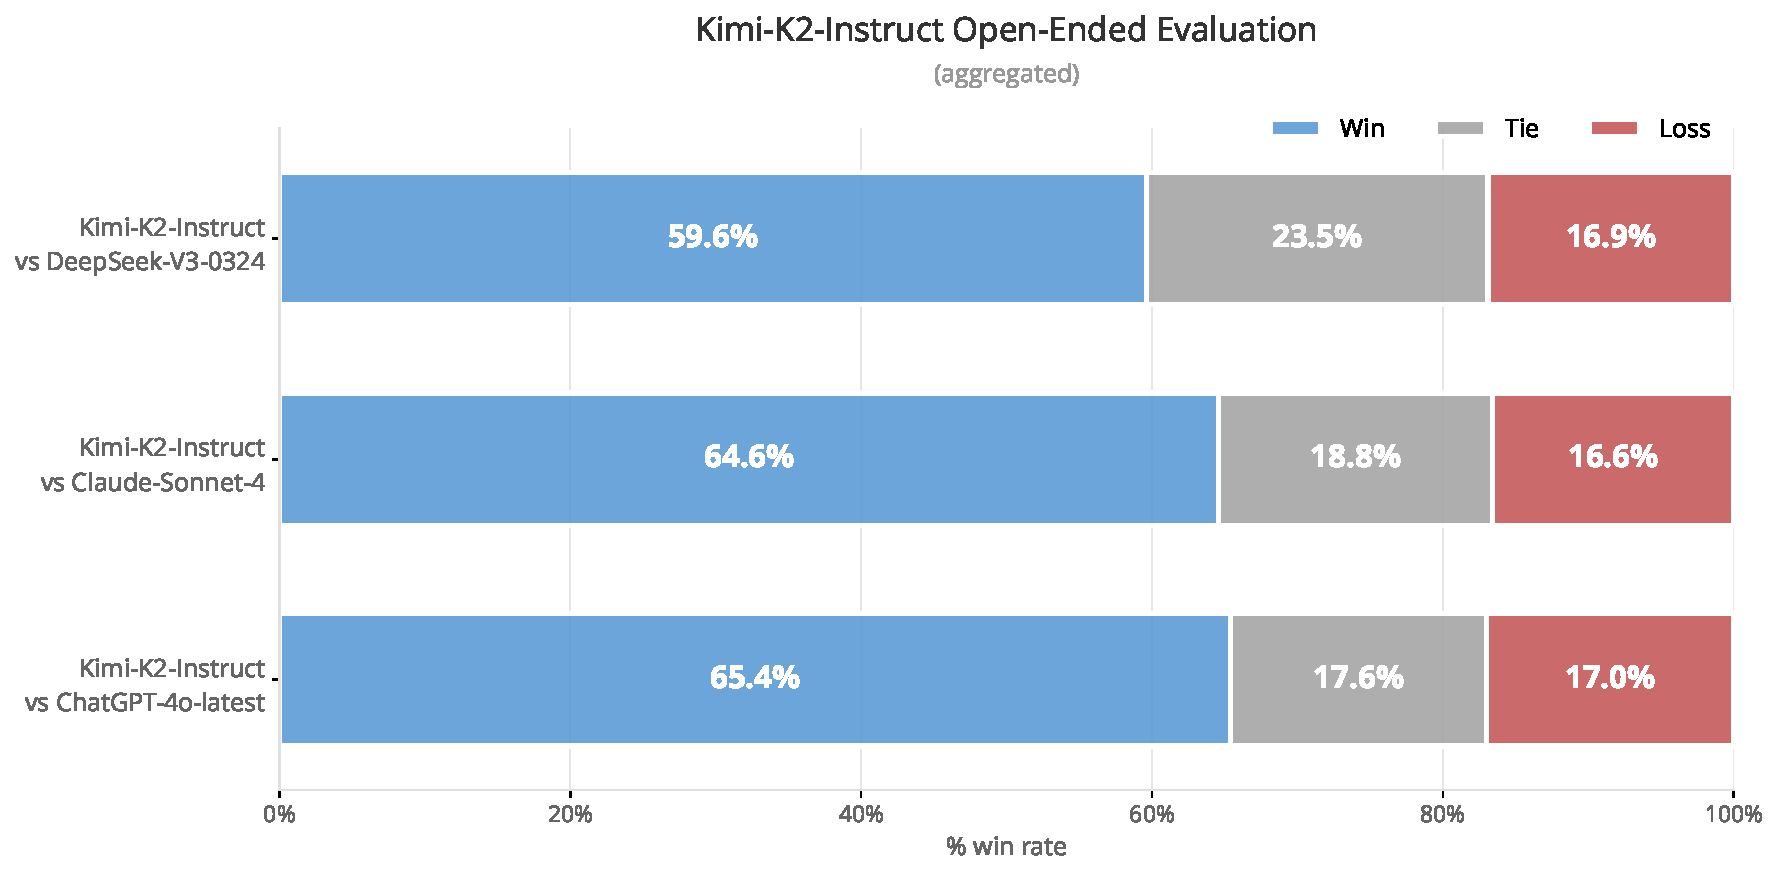
\includegraphics[width=0.8\linewidth]{figures/posttrain_inhouse_eval.pdf}
    \caption{Chinese in-house benchmark evaluation.}
    \label{fig:posttrain_inhouse_eval}
\end{figure}


















\section{QK-Clip Does Not Impair Model Quality}
\label{sec:qkclip_harmless}

The QK-Clip design follows a \textbf{minimal intervention principle}: it activates only when necessary, and deactivates after training stabilizes. Empirical evidence and analysis converge on its negligible impact on model quality.

\paragraph{Small-Scale Ablations}

\begin{figure}[t]
\centering
\begin{minipage}[t]{0.48\textwidth}
  \centering
  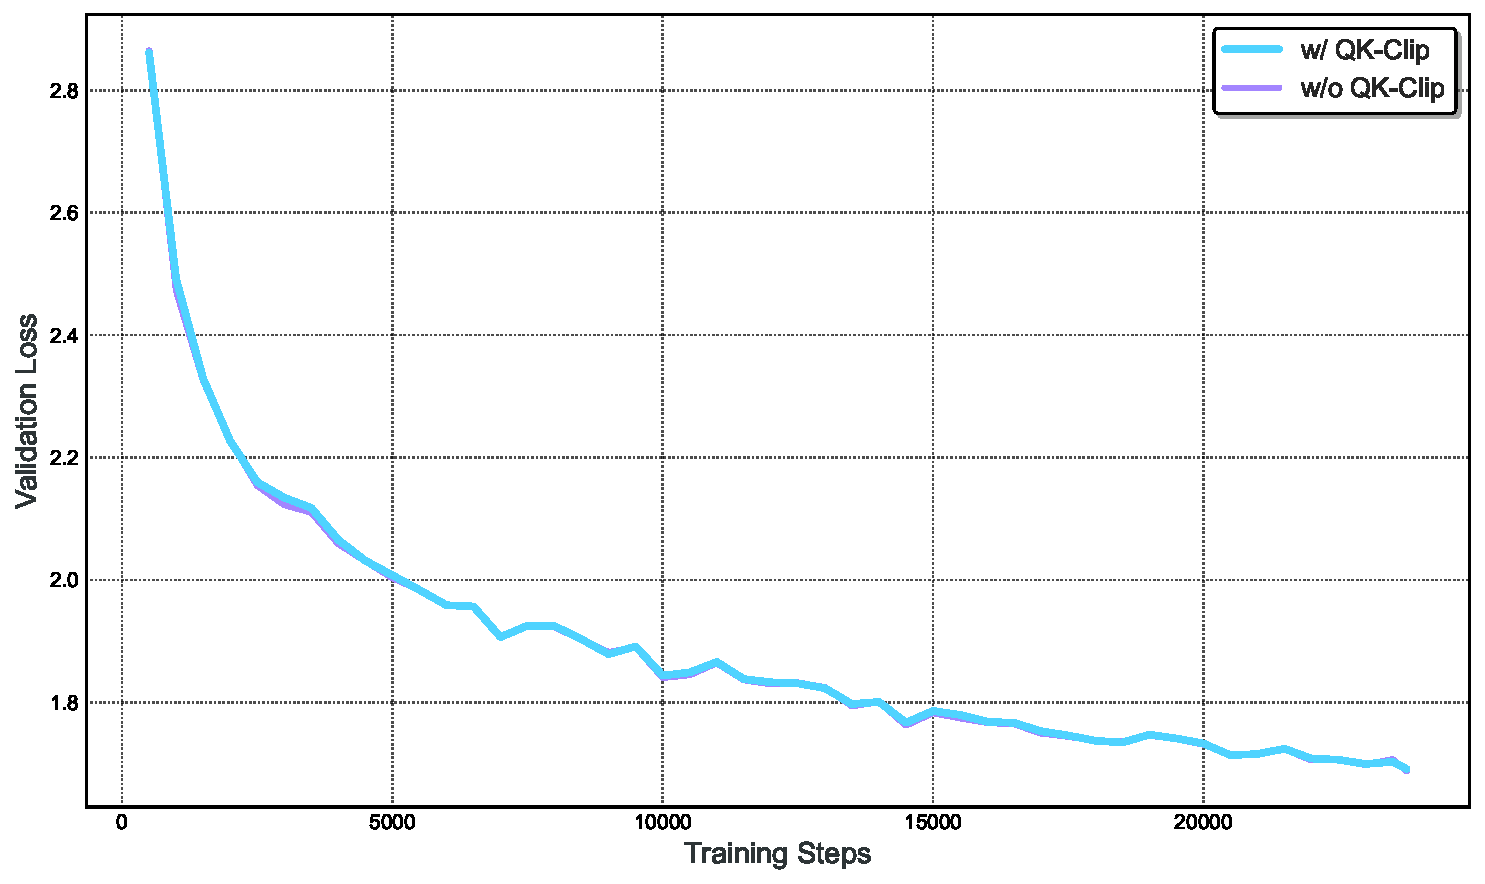
\includegraphics[width=\linewidth]{figures/muon-qkclip_vs_noclip.pdf}
  \caption{Applying QK-Clip to Muon in a small-scale setting with an aggresive threshold ($\tau$ = 30) has negligible impact on loss, indicating that it is a safe and effective method for constraining attention logits.}

  \label{fig:mini_muonclip_loss}
\end{minipage}\hfill
\end{figure}


We train two small-scale 0.5B activated and 3B total parameters MoE models, one with vanilla Muon and the other with MuonClip using a low clipping threshold ($\tau = 30$). 
As shown in Figure~\ref{fig:mini_muonclip_loss}, applying MuonClip has negligible effects on the loss curve, indicating that even aggressive clipping does not impair convergence or training dynamics with MuonClip. This demonstrates that MuonClip is a safe and effective method for bounding attention logits without degrading model performance. Furthermore, evaluation on downstream tasks reveals no statistically significant degradation in performance. These results collectively demonstrate that MuonClip is a safe and effective method for bounding attention logits without compromising model quality.


\paragraph{Self-deactivation}
In Kimi K2, QK-Clip was only transiently active:
\begin{itemize}
  \item \textbf{Initial {70000} steps:} $12.7\%$ of attention heads triggered QK-Clip for at least once, clamping $S_{\max}$ to $100$.
  \item \textbf{Post-{70000} steps:} All heads at some point reduced their $S_{\max}$ below $100$, rendering QK-Clip inactive.
\end{itemize}

When QK-Clip is active, it is applied per-head (rather
than per-layer) to minimize potential over-regularization on other heads.
After training stabilizes, QK-clip is deactivated and has no effect at all.


\section{Why Muon is More Prone to Logit Explosion}

Logit explosion occurs when the largest pre-softmax attention score
\begin{equation}
S_{\max} = \max_{i,j} \bigl(q_i^{\vphantom{\top}}\! \cdot k_j\bigr)
\end{equation}
grows unboundedly during training.  Since
\begin{equation}
|q_i \!\cdot\! k_j| \le \|q_i\|\|k_j\| \le \|x_i\|\|x_j\|\|\mathbf W_q\|\|\mathbf W_k\|,
\end{equation}
and RMS-Norm keeps $\|x_i\|\|x_j\|$ bounded, the phenomenon is primarily driven by the growing spectral-norm of $\mathbf W_q$ or $\mathbf W_k$.  Empirically, we found that Muon is more susceptible to logit explosion. We give our hypothesis below.

\paragraph{Structural difference in updates}
Muon produces a weight update coming from the $\mathrm{msign}$ operation; as a result, \emph{all} singular values of the update matrix are equal --- its effective rank is full.  
In contrast, a typical update matrix produced by Adam exhibits a skewed spectrum: a few large singular values dominate, and the effective rank is low.  This low-rank assumption for Adam is not new; higher-order muP makes the same assumption.

Such phenomenon is verified on the 16\,B Moonlight model, which shows weights trained with Muon exhibit higher \emph{singular-value entropy} (i.e.\ higher effective rank) than those trained with Adam, corroborating the theoretical intuition.

\paragraph{SVD formulation}  
Let the parameter matrix at step $t-1$ have the singular value decomposition
\begin{equation}
\mathbf W_{t-1}=\sum_i \sigma_i\,u_i v_i^{\top}
\end{equation}
We write the update matrices as
\begin{align}
\Delta\mathbf W_t &= \sum_j \bar\sigma\,\bar u_j \bar v_j^{\top}
\end{align}  
The next parameter update is therefore
\begin{align}
\mathbf W_t \leftarrow \sum_i \sigma_i u_i v_i^{\top} + \sum_j \bar\sigma\,\bar u_j \bar v_j^{\top}
\end{align}

In Muon, as both the weights and the updates have a higher effective rank than Adam, we hypothesize there is a higher probability for singular-vector pair $u_i v_i^{\top}$ to align with $\bar u_j \bar v_j^{\top}$. This could cause the corresponding singular value of $\mathbf W_t$ to increase additively.

\paragraph{Attention-specific amplification}  
Attention logits are computed via the bilinear form
\begin{equation}
q_i\cdot k_j=(x_i \mathbf W_q)\cdot (x_j \mathbf W_k).
\end{equation}
The product $\mathbf W_q\mathbf W_k^{\top}$ squares the spectral norm, so any singular-value increase in either matrix is compounded.  Muon's tendency to enlarge singular values therefore translates into a higher risk of logit explosion.



\section{K2 Critic Rubrics for General RL}

\subsection{Core Rubrics}
\label{sec:k2-critic-creteria}
\begin{itemize}
    \item \textbf{Clarity and Relevance:} Assesses the extent to which the response is succinct while fully addressing the user's intent. The focus is on eliminating unnecessary detail, staying aligned with the central query, and using efficient formats such as brief paragraphs or compact lists. Unless specifically required, long itemizations should be avoided. When a choice is expected, the response should clearly offer a single, well-defined answer.

    \item \textbf{Conversational Fluency and Engagement:} Evaluates the response's contribution to a natural, flowing dialogue that extends beyond simple question-answering. This includes maintaining coherence, showing appropriate engagement with the topic, offering relevant observations or insights, potentially guiding the conversation constructively when appropriate, using follow-up questions judiciously, handling hypothetical or personal-analogy queries gracefully, and adapting tone effectively to suit the conversational context (e.g., empathetic, formal, casual).

    \item \textbf{Objective and Grounded Interaction:} Assesses the response's ability to maintain an objective and grounded tone, focusing squarely on the substance of the user's request. It evaluates the avoidance of both metacommentary (analyzing the query's structure, topic combination, perceived oddity, or the nature of the interaction itself) and unwarranted flattery or excessive praise directed at the user or their input. Excellent responses interact respectfully but neutrally, prioritizing direct, task-focused assistance over commentary on the conversational dynamics or attempts to curry favor through compliments.
\end{itemize}

\subsection{Prescriptive Rubrics}
\label{sec:k2-must-not-creteria}
\begin{itemize}
    \item \textbf{Initial Praise:} Responses must not begin with compliments directed at the user or the question (e.g., ``That's a beautiful question'', ``Good question!'').
    \item \textbf{Explicit Justification:} Any sentence or clause that explains why the response is good or how it successfully fulfilled the user's request. This is different from simply describing the content.
\end{itemize}

\subsection{Limitations}
One potential side effect of this evaluation framework is that it may favor responses that appear confident and assertive, even in contexts involving ambiguity or subjectivity. This stems from two key constraints in the current rubric:
\begin{itemize}
    \item \textbf{Avoidance of Self-Qualification:} The prescriptive rules prohibit self-assessments, explicit disclaimers, or hedging language (e.g., ``this may not be accurate'', ``I might be wrong''). While these phrases can reflect epistemic humility, they are often penalized as non-informative or performative.
    \item \textbf{Preference for Clarity and Singularity:} The rubric reward direct, decisive answers when users ask for a recommendation or explanation. In complex or open-ended scenarios, this may disincentivize appropriately cautious or multi-perspective responses.
\end{itemize}
As a result, the model may occasionally overstate certainty in areas where ambiguity, nuance, or epistemic modesty would be more appropriate. Future iterations of the framework may incorporate more fine-grained handling of calibrated uncertainty.


\section{Engine Switching Pipeline for RL Training}
\label{sec:k2-rl-update-appendix}

\begin{figure}[htb]
   \centering
   \begin{subfigure}[b]{0.7\textwidth}
       \centering
       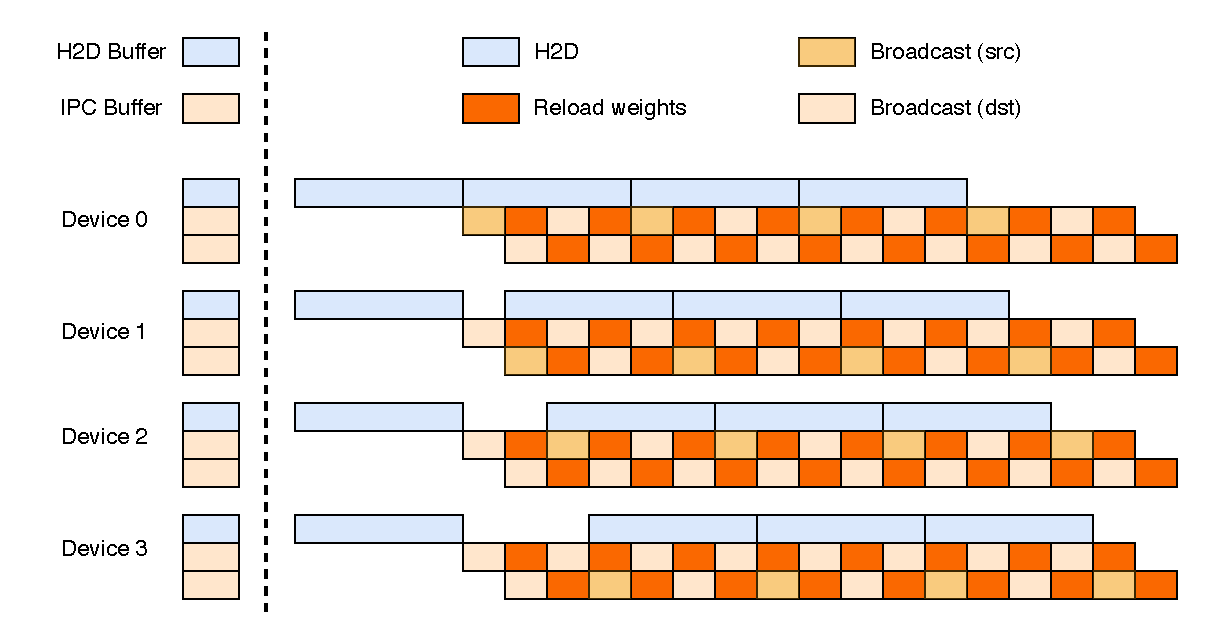
\includegraphics[width=1\linewidth]{figures/new-rl-reload-3-stage-pipeline.pdf}
       \caption{Theoretical perfect three-stage pipeline weight update}
       \label{fig:mshrl:update-weight}
   \end{subfigure}
   \begin{subfigure}[b]{0.4\textwidth}
        \centering
        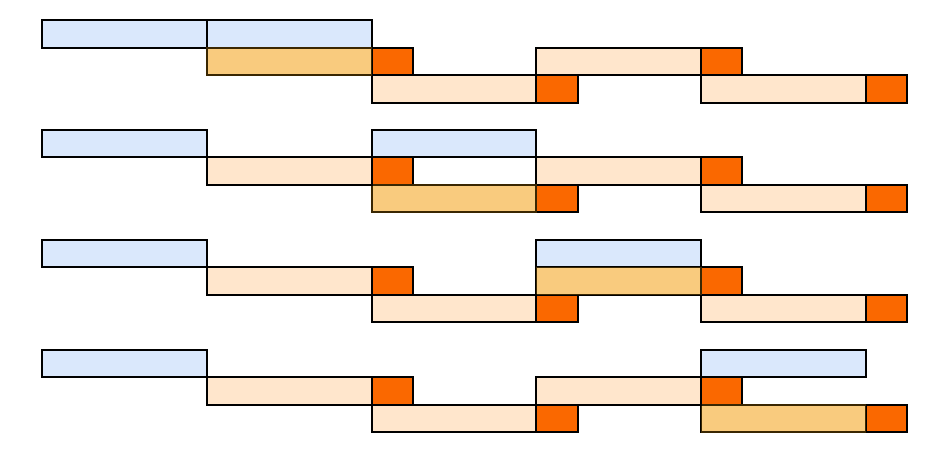
\includegraphics[width=\textwidth]{figures/new-rl-reload-pcie-bound-3-stage-pipeline.pdf}
        \caption{A PCIE bounded three-stage pipeline}
        \label{fig:mshrl:update-overhead}
   \end{subfigure}
   \hspace{0.02\textwidth}
   \begin{subfigure}[b]{0.35\textwidth}
        \centering
        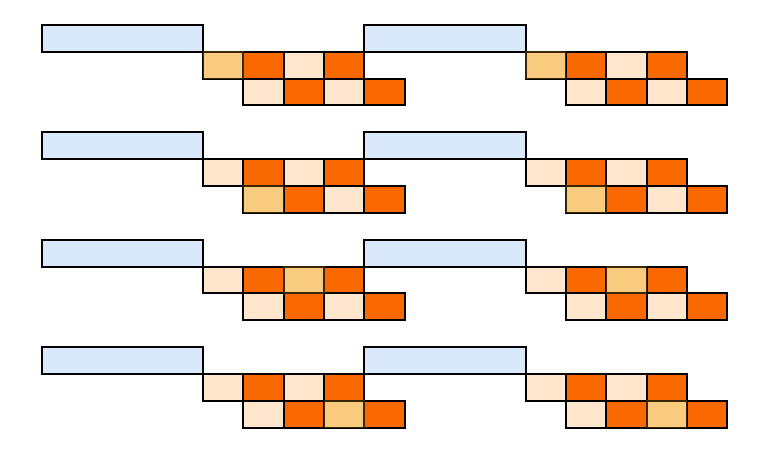
\includegraphics[width=\textwidth]{figures/new-rl-reload-2-stage-pipeline.pdf}
        \caption{Fixed two-stage pipeline}
        \label{fig:mshrl:update-final}
   \end{subfigure}
   \caption{pipeline for RL weight update}
   \label{fig:mshrl-fixed-update}
\end{figure}

The \emph{checkpoint engine} manages three equal-size device buffers on each GPU: an H2D buffer for loading the offloaded model parameters, and two IPC buffers for GPU-to-GPU broadcast.
The IPC buffers are shared to inference engines, allowing it to directly access the same physical memory.
 These three buffers allow us to arrange the three steps in a pipeline.
 
\paragraph{Theoretical three-stage pipeline.}  
As illustrated in Figure~\ref{fig:mshrl:update-weight}, a three-stage pipeline is introduced.
(1) \emph{H2D}: a shard of the latest weights is copied into the H2D buffer asynchronously.
(2) \emph{Broadcast}: Once the copy completes, the shard will be copied to one IPC buffers and broadcast to all devices.
(3) \emph{Reload}: Inference engines simultaneously load parameters from the other IPC buffer.

\paragraph{Two-stage pipeline due to PCIe saturation.}  
On NVIDIA H800 clusters, concurrent H2D and broadcast saturate the shared PCIe fabric, collapsing the three stages into a sequential procedure (Figure~\ref{fig:mshrl:update-overhead}).  
We therefore adopt a simpler, two-stage scheme (Figure~\ref{fig:mshrl:update-final}): (1) All devices perform a single, synchronous H2D transfer. (2) The broadcast and reload proceed in parallel.

The two-stage pipeline will be bound by multiple synchronous H2D copy operations. But in large scale devices, model will be split into small shards, the entire parameter set fits into the H2D buffer in one transfer, the overhead will disappear.

By overlapping H2D, Broadcast, and Reload weights, we can obtain a high bandwidth to reshard the weights from train engines to all inference engines.

